\subsubsubsection{low\_degree\_interpolation}

\hspace*{\fill}

\indent InterpolationGate is used for the interpolation of a polynomial, whose points are a (base field) coset of the multiplicative subgroup 
with the given size, and whose values are extension field elements. As for LowDegreeInterpolationGate,  all constraints are degree <= 2, 
low degree is a tradeoff for more gates (than HighDegreeInterpolationGate).

LowDegreeInterpolationGate trace is shown in \figref{fig:low-degree-interpolation}.

\begin{figure}[!ht]
    \centering
    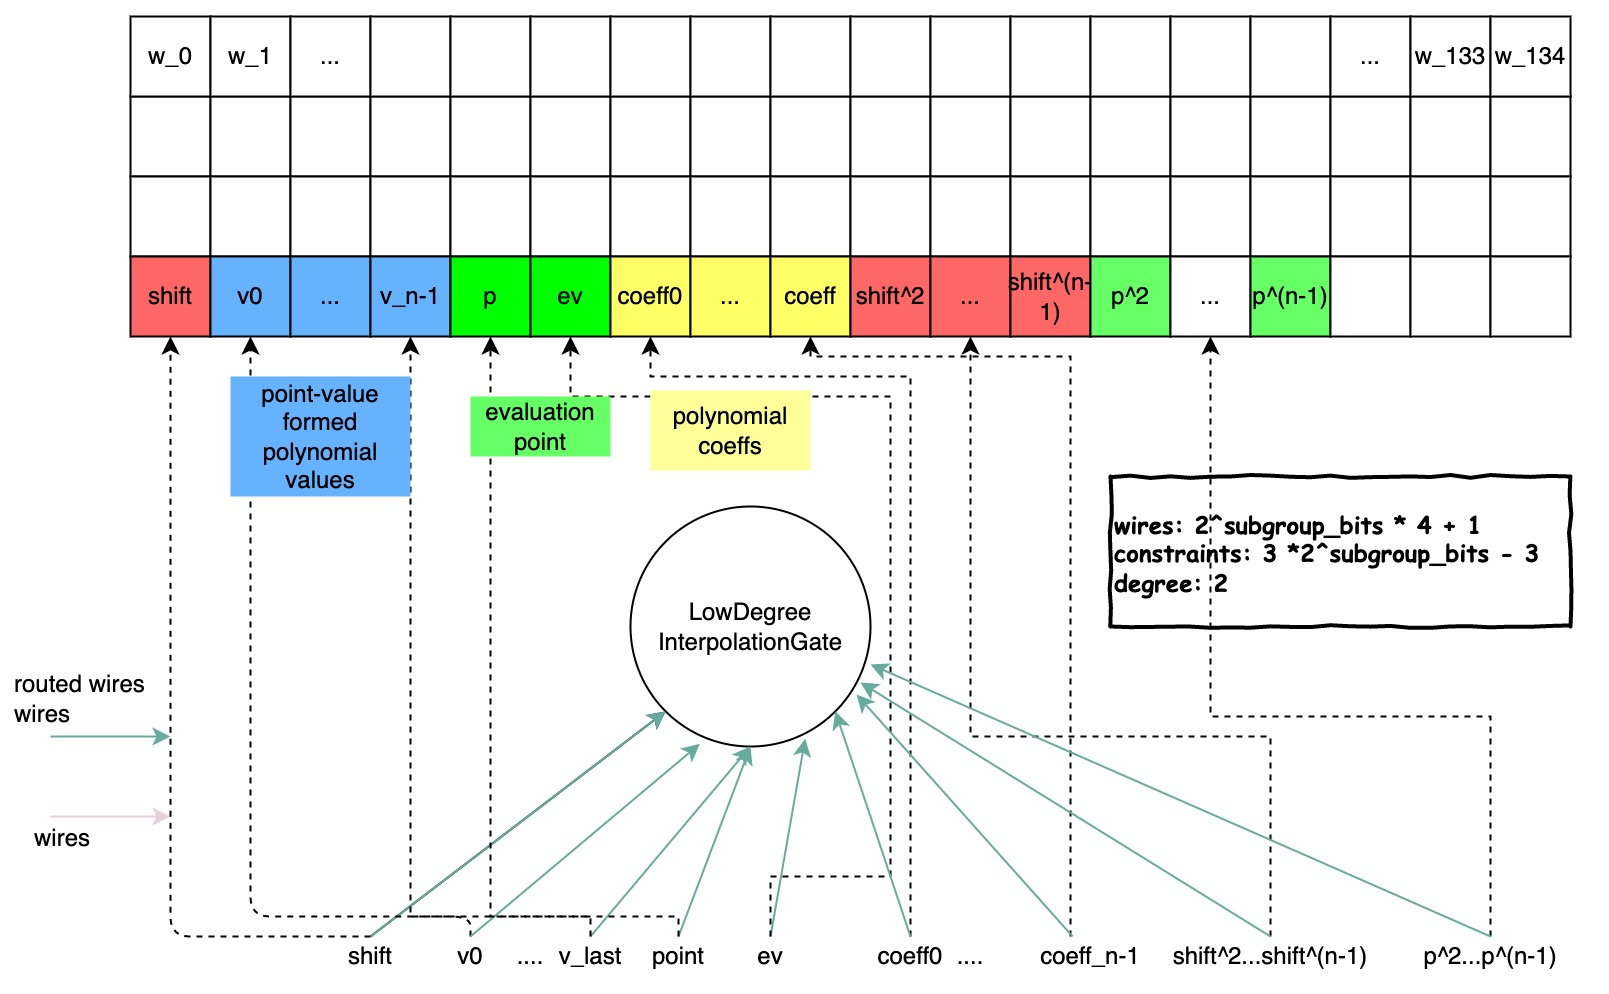
\includegraphics[width=0.6\textwidth]{gates/low_degree_interpolation.jpeg}
    \caption{LowDegreeInterpolationGate}
    \label{fig:low-degree-interpolation}
\end{figure}

Constraints as follows:
\begin{itemize}
    \item Constrain powers of shift, from $\text{shift}^2$ to $\text{shift}^{n-1}$, a total of $2^{\text{subgroup\_bits}}-2$ constraints.
    \begin{lstlisting}[language=rust]
for i in 1..self.num_points() - 1 {
    constraints.push(powers_shift[i - 1] * shift - powers_shift[i]);
}
    \end{lstlisting}
    \item Bring each point (from the point-value pairs) into the coefficient polynomial to compute the computed\_value 
    and compare the constraint with the value (from the point-value pairs). -- A total of $2^{\text{subgroup\_bits}}$ constraints.
    \item Constrain powers of evaluation point. -- A total of $2^{\text{subgroup\_bits}}-2$ constraints.
    \item Evaluate the coefficient-form polynomial at the evaluation point and constrain it. -- 1 constraint.
\end{itemize}

As can be seen from the above constraint description, the number of constraints is $3 \cdot 2^{\text{subgroup\_bits}}-3$, degree of LowDegreeInterpolationGate is 2.
